% ---------------------------------------------------------------------------
%  Methods for: Frequency-resolved active-space downfolding of the
%  electron-defect vertex, and the defect spectral function from it.
%
%  REVTeX 4.2 / APS.  Set for PRX; for PRL use this as Supplemental Material
%  (swap prx -> prl and add \documentclass[...,supplement]{}).
%  Compile: pdflatex methods && bibtex methods && pdflatex methods x2
% ---------------------------------------------------------------------------
\documentclass[aps,prx,reprint,superscriptaddress,nofootinbib,longbibliography]{revtex4-2}

\usepackage{amsmath,amssymb,bm}
\usepackage{graphicx}
\usepackage{booktabs}
\usepackage[colorlinks=true,linkcolor=blue,citecolor=blue,urlcolor=blue]{hyperref}
\graphicspath{{../docs/assets/}}

\newcommand{\dV}{\Delta V}
\newcommand{\Vt}{\widetilde{V}}
\newcommand{\Rd}{\mathbf{R}_{\rm def}}
\newcommand{\kk}{\mathbf{k}}
\newcommand{\rr}{\mathbf{r}}
\newcommand{\RR}{\mathbf{R}}
\newcommand{\qq}{\mathbf{q}}
\newcommand{\GG}{\mathbf{G}}
\newcommand{\meV}{\;\mathrm{meV}}

\begin{document}

\title{Methods: frequency-resolved active-space downfolding of the
electron--defect vertex and the defect spectral function}

\author{R.\ Guo}
\affiliation{The University of Texas at Austin}

\date{\today}

\begin{abstract}
We describe a first-principles route from a defect supercell to the
electron--defect spectral function $A(\kk,\omega)$ of an isolated defect on an
arbitrarily fine $k$-mesh. The scattering vertex is downfolded onto a small
active manifold by an exact Feshbach partition, with the rest-space
contribution resummed to all orders and resolved in frequency by a block
Lanczos continued fraction. The dressed vertex is carried to fine $k$ by a
pair-Wannier transform, and the $T$-matrix is closed on a real-space cluster
whose dimension is independent of the fine mesh. Each step is gated by a
quantitative test: an operator-level identity, level-by-level comparison with a
supercell reference at two supercell $k$-points, a leave-one-out test of the
interpolation, and closure of the end-to-end chain onto the directly
diagonalized quasiparticle levels to $0.4\meV$.
\end{abstract}

\maketitle

\section{Overview}

The object of interest is the electron--defect self-energy of a dilute,
randomly distributed defect,
\begin{equation}
  \Sigma^{\rm ed}_{mn}(\kk,\omega) = n_d\, T_{mn}(\kk,\kk;\omega),
  \label{eq:sigmaed}
\end{equation}
and the spectral function that follows from it,
\begin{equation}
  A(\kk,\omega) = -\frac{1}{\pi}\,\mathrm{Im}\,\mathrm{Tr}
  \big[\omega + i\eta - H_0(\kk) - \Sigma^{\rm ed}(\kk,\omega)\big]^{-1}.
  \label{eq:Akw}
\end{equation}
Three obstacles stand between a supercell calculation and
Eqs.~\eqref{eq:sigmaed}--\eqref{eq:Akw}. First, the scattering must be summed
to all orders, not truncated at the Born level, because a defect that binds a
state is not perturbative. Second, the sum must be resolved in frequency:
freezing it at a reference energy is exact only there. Third, a supercell fixes
both the defect concentration and the $k$-mesh, whereas
Eq.~\eqref{eq:sigmaed} requires the isolated limit and a mesh dense enough to
resolve $A(\kk,\omega)$.

The method addresses the three in sequence. Section~\ref{sec:downfold} splits
the Hilbert space and eliminates everything outside a small active manifold
exactly. Section~\ref{sec:vertex} constructs the bare vertex on the primitive
grid and states the conditions under which that construction is exact.
Section~\ref{sec:lanczos} resums the eliminated space to all orders and to
arbitrary $\omega$. Section~\ref{sec:wannier} carries the result to fine $k$,
and Sec.~\ref{sec:tmatrix} closes the $T$-matrix in real space, where the
concentration becomes a free parameter decoupled from the mesh.
Section~\ref{sec:validation} collects the tests.

Throughout, the illustrative system is a monolayer MoS$_2$ with a relaxed
sulfur vacancy (V$_{\rm S}$), and, where stated, the isovalent substitutions
O$_{\rm S}$ and Se$_{\rm S}$.


\section{Active/rest partition and the exact downfolding identity}
\label{sec:downfold}

Let $P_A$ project onto an active manifold $A$ --- $n_b$ Bloch bands of the
pristine crystal at each of $N_k$ points of a coarse mesh, so
$N_A = n_b N_k$ --- and let $P_R = 1 - P_A$. With $H = H_0 + \dV$, where
$H_0$ is the pristine Kohn--Sham Hamiltonian and $\dV$ the defect potential,
Feshbach--L\"owdin partitioning of $(\omega - H)^{-1}$ gives the projected
Green function on $A$ \emph{exactly},
\begin{equation}
  G_A(\omega) = \big[\omega - \varepsilon_A - \Vt(\omega)\big]^{-1},
  \label{eq:GA}
\end{equation}
with the dressed vertex
\begin{equation}
  \Vt(\omega) = \frac{1}{N_k}\Big[ M_{AA} + \Sigma^R(\omega) \Big],
  \qquad
  M_{ab} = \langle \psi_a | \dV | \psi_b \rangle ,
  \label{eq:Vtilde}
\end{equation}
and the rest self-energy
\begin{equation}
  \Sigma^R(\omega) = V_{AR}\,\big[\omega - P_R H P_R\big]^{-1} V_{RA}.
  \label{eq:SigmaR}
\end{equation}
Equation~\eqref{eq:SigmaR} contains \emph{every} path that leaves $A$, scatters
an arbitrary number of times within $R$, and returns --- all orders in $\dV$
restricted to $R$, zeroth order in $A$. The complementary paths, those that
re-enter $A$, are generated by inverting Eq.~\eqref{eq:GA} or, equivalently, by
the ladder of Sec.~\ref{sec:tmatrix}. Because $P_A P_R = 0$, no path is
counted twice; this is the structural reason a $T$-matrix built on $\Vt$ with
an active-space propagator requires no subtraction.

Two consequences are used later. (i) Since $\Sigma^R$ depends on $\omega$, the
spectral weight carried by $A$ is less than unity, with the quasiparticle
renormalization $Z = [1 - \partial_\omega \Vt]^{-1}$; this must be reported when
$A$-space spectral weights are compared with total ones. (ii) The factor
$1/N_k$ in Eq.~\eqref{eq:Vtilde} is the Born--von-K\'arm\'an normalization: a
calculation on an $N_k$-point mesh describes one defect per $N_k$ primitive
cells. $N_k$ is therefore not only a sampling parameter but also the dilution,
a point we return to in Sec.~\ref{sec:freegrid}.


\section{The defect vertex on the primitive grid}
\label{sec:vertex}

\subsection{Folding the supercell potential}

$\dV$ is obtained as the difference of the self-consistent local potentials of
a defect supercell and the corresponding pristine supercell, aligned in the
vacuum. It is represented on the supercell real-space grid. The matrix element
between primitive-cell Bloch states requires it folded onto the primitive grid
with the exact momentum transfer,
\begin{equation}
  V_\qq(\rr) = \sum_{\RR \in \rm cell}
  \dV(\rr + \RR)\, e^{i\qq \cdot (\rr + \RR)},
  \qquad \qq = \kk' - \kk,
  \label{eq:fold}
\end{equation}
where $\RR$ runs over the primitive lattice vectors contained in the supercell
box. Equation~\eqref{eq:fold} is evaluated on the fly for each pair, with the
phase running over the \emph{whole} box and $\qq$ taken exactly; wrapping
$\qq$ into the first Brillouin zone without the compensating phase would
introduce a spurious factor. The implementation follows the convention of
Ref.~\onlinecite{LuBernardi2020}.

\subsection{Commensurability of the fold}

The sum in Eq.~\eqref{eq:fold} is realized as a real-space modulo map,
$r^{\rm cell}_i \to r^{\rm cell}_i \bmod n^{\rm prim}_i$. This is exact only if
\begin{equation}
  n^{\rm cell}_i = N^{\rm sc}_i \, n^{\rm prim}_i
  \qquad \text{on every axis,}
  \label{eq:commensurate}
\end{equation}
i.e.\ the ratio must \emph{be} the supercell multiplicity, not merely an
integer. The failure is silent: in-gap states still appear at roughly the right
energies while $C_3$-degenerate doublets split by tens of meV and
$\lVert \Vt \rVert$ changes by tens of percent. A merely integral ratio fails
just as badly --- a $240$-point cell of a $6\times$ supercell folded onto a
$30$-point primitive grid (ratio $8$) returned $15$ states in a window that
holds $5$. Degeneracy splitting of a symmetric defect is the cheap
fingerprint; on commensurate grids the $C_3$ pairs here are degenerate to
$0$--$4\,\mu$eV. The code prints both grids and the detected multiplicity and
aborts when Eq.~\eqref{eq:commensurate} fails.

Equation~\eqref{eq:commensurate} can be satisfied from either side. Rather than
refine the primitive grid to match a fine potential grid, we band-limit the
potential onto a coarser commensurate grid by truncation in $\GG$-space, which
is exact for every Fourier component the coarse grid supports. For the case
studied, $240\times240\times300 \to 162\times162\times216$ discards
$4\times10^{-8}$ of the spectral weight of $\dV$ and pairs with the natural
$27\times27\times216$ primitive grid; the cost of Eq.~\eqref{eq:fold} falls in
proportion to the grid, and quasiparticle levels move by $\le 0.1\meV$.

\subsection{The $k$-mesh is free; $N_k$ is the dilution}
\label{sec:freegrid}

The supercell is a container that captures one isolated defect, not a
periodicity we wish to impose. Because the phase in Eq.~\eqref{eq:fold} runs
over the whole box, $V_\qq$ is the finite-box transform of a \emph{localized}
$\dV$ and is defined, and generically nonzero, for arbitrary $\qq$. The
$k$-mesh therefore need not match the supercell.

The distinction is quantitative. Treating the box as a periodicity would set
$\langle \psi_\kk | \dV | \psi_{\kk'} \rangle = 0$ unless
$\kk - \kk' \in \{\GG_{\rm sc}\}$. Measured on a $12\times12$ mesh against a
$6\times6$ box, matrix elements between $k$-points differing by a
non-supercell vector reach $0.975$ of the largest within-supercell one: the
periodic reading would discard most of the scattering channels.

Two inequivalent calculations therefore share the name ``$12\times12$'':
\begin{enumerate}
\item[(a)] \emph{Coset-decomposed.} Since $\dV$ of a strictly periodic array
cannot connect them, the mesh splits into $(N_k/N^{\rm sc})^2$ cosets of the
supercell reciprocal lattice, each an independent run of the designed size, and
each folding to one supercell $k$-point. The dilution stays at $1/N^{\rm sc}$,
which is what makes it comparable to a supercell calculation. This is a
validation device (Sec.~\ref{sec:truth}), not the physics target.
\item[(b)] \emph{Direct.} One run on the full mesh: one defect per $N_k$ cells,
with $\qq$ resolved throughout the zone. This is the dilute limit the method
targets.
\end{enumerate}
The two agree where they must: the coset-diagonal blocks of the direct
$144$-$k$ vertex reproduce the four shifted $36$-$k$ runs to $2\times10^{-6}$
on a block scale of $66$, compared gauge-invariantly through block eigenvalues.


\section{The rest self-energy by block Lanczos}
\label{sec:lanczos}

This section records the algorithm in full. An \emph{active label} is a pair
$a=(n,\kk_i)$ of band and coarse momentum, $N_A$ their number; a
\emph{bundle} $|\chi\rangle$ is one algebraic vector with a plane-wave
component at \emph{every} coarse channel, $\chi_{\kk'}(\GG,\sigma)$, of total
length $N^{\sigma}_{\rm pw}N_k$ ($\sigma$: spinor component;
$N^{\sigma}_{\rm pw}=2N_{\rm pw}$ for $n_{\rm pol}=2$). The bundle inner
product sums over channels,
$\langle\chi|\xi\rangle=\sum_{\kk'\GG\sigma}
\chi^{*}_{\kk'}(\GG,\sigma)\,\xi_{\kk'}(\GG,\sigma)$;
every orthogonality statement below refers to it.

\subsection{Source block: construction and projection}

The resolvent \eqref{eq:SigmaR} is needed only between the $N_A$ sources
\begin{equation}
  |\chi_a\rangle = P_R\, \dV\, |\psi_a\rangle ,
  \qquad P_R = 1-P_A,\quad
  P_A=\sum_{b\in A}|\psi_b\rangle\langle\psi_b| .
  \label{eq:source}
\end{equation}
Three details fix the implementation.
(i) $\dV|\psi_a\rangle$ uses the exact-$q$ fold of Sec.~\ref{sec:fold}: the
state resident at channel $\kk_i$ scatters into \emph{every} channel $\kk'$
with the folded potential $V_{\kk_i-\kk'}(\rr)$ of Eq.~\eqref{eq:applydV};
no momentum is wrapped to a supercell zone. The nonlocal
(Kleinman--Bylander) difference is added per output channel,
$\sum_{\mu\nu}|\beta^{\kk'}_{\mu}\rangle D_{\mu\nu}
\langle\beta^{\kk_i}_{\nu}|\psi_a\rangle$ with
$D=D^{\rm def}\ominus D^{\rm prist}$ built from the defect and pristine atom
lists; for $n_{\rm pol}=2$ the local fold acts diagonally on the two spinor
components while $D$ carries the $2\times2$ spin blocks of
$d^{\rm so}_{\mu\nu}$ (spin-diagonal $d_{\mu\nu}$ for scalar
pseudopotentials).
(ii) $P_R$ is applied channel-wise, subtracting the active states of each
channel. The active states are exact eigenstates of the same Kohn--Sham $H$,
so $[H,P_A]=0$ and the Krylov space below stays in $\mathrm{ran}\,P_R$ up to
roundoff; the projector is nevertheless re-applied with each
reorthogonalization as numerical hygiene.
(iii) The sources are assembled and QR-factorized \emph{in the bundle inner
product},
\begin{equation}
  \big[\,\chi_1\;\cdots\;\chi_{N_A}\big] = Q_1 R_0 ,
  \qquad Q_1^{\dagger}Q_1=\openone_{N_A},
  \label{eq:qr0}
\end{equation}
with $R_0$ ($N_A{\times}N_A$, upper triangular) stored: the sources enter the
final resolvent only through it, and its singular values are those of
$V_{RA}$ (the basis of the rank compression discussed in
Sec.~\ref{sec:cost}).

\subsection{Block recurrence}

With $Q_0\equiv0$, steps $j=1,\dots,N_S$ perform
\begin{align}
  W &= H\,Q_j ,\label{eq:happly}\\
  A_j &= Q_j^{\dagger}W
     \quad(\text{Hermitian; } \|A_j-A_j^{\dagger}\|\sim10^{-14}
     \text{ monitored per step}),\nonumber\\
  W &\leftarrow W - Q_jA_j - Q_{j-1}B_{j-1}^{\dagger},\nonumber\\
  W &\leftarrow W - \sum_{l=\max(1,\,j-m)}^{j} Q_l\,(Q_l^{\dagger}W)
     \quad(\text{window }m),\label{eq:reorth}\\
  Q_{j+1}B_j &= \mathrm{qr}(W)\quad(B_j\text{ upper triangular}).
  \label{eq:qrj}
\end{align}
$H$ in \eqref{eq:happly} is the untouched Kohn--Sham Hamiltonian of the
pristine primitive cell, applied channel-diagonally: kinetic term in
$\GG$-space, one FFT pair for the local potential, a projector
\textsc{zgemm} for the nonlocal part. $\dV$ never appears after the source
step --- the defect enters $\Sigma^R$ only through $R_0$. The coefficient
pair $(A_j,B_j)$ is appended to the chain file; bundles are discarded as the
window advances. Applying $\dV$ (source step and the operator-identity gate
below) is the cost driver: by Eq.~\eqref{eq:applydV} every output channel
couples to every source channel, a triple loop over grid points, channels
and columns.

Before the first step the code verifies the \emph{operator identity}
$\langle\psi_b|\dV|\psi_a\rangle$ (recomputed by the fold machinery on probe
columns) against the independently produced Born block $M_{AA}$; agreement at
the $10^{-11}$ level is required and doubles as a cross-code closure when
$M_{AA}$ comes from EDI. Failures of this gate have caught every interface
and convention bug encountered during development.

\subsection{Reorthogonalization: the rolling window}

The classic Lanczos hazard --- ghost eigenvalues from lost orthogonality ---
sets in only when a Ritz value converges (Paige). For the chains used here
($N_S\le32$ blocks of width $N_A$ in a space of dimension
$N^{\sigma}_{\rm pw}N_k\sim10^{6}$--$10^{7}$) no Ritz pair converges, and a
window of $m$ blocks in \eqref{eq:reorth} suffices. This was verified rather
than assumed: against full reorthogonalization, $m=2$ reproduces the chain
matrices to $3\times10^{-14}$ on a scale of $31$, the physical levels
bit-for-bit, and the global orthogonality
$\max|Q^{\dagger}Q-\openone|=6.0\times10^{-9}$ identical to four digits;
$m=1$ agrees with $m=2$ to $0.000000$ meV. The window replaces the full
block store ($N_S{+}1$ blocks) by $m{+}1$ slots reused modulo $m{+}1$;
together with the in-flight work block this sets the memory floor of the
method at $(m{+}2)$ bundles of width $N_A$ (Sec.~\ref{sec:cost}).

\subsection{Continued fraction and evaluation}

For any complex $\omega$ the resolvent follows from the block continued
fraction, evaluated from the bottom of the chain,
\begin{equation}
  S_j = \big[\omega - A_j - B_j^{\dagger} S_{j+1} B_j \big]^{-1},
  \qquad
  \Sigma^R(\omega) = \frac{R_0^{\dagger} S_1(\omega) R_0}{N_k}.
  \label{eq:cf}
\end{equation}
The inverse is constructed, never expanded, so there is no convergence-radius
condition: a dressed rest state that a Neumann ladder would fail to converge is
carried exactly. One chain serves every $\omega$ and every broadening.

Evaluation details. The recursion is initialized at the bottom,
$S_{N_S}=[\omega-A_{N_S}]^{-1}$, and swept upward; each $\omega$ costs
$N_S$ Hermitian solves of size $N_A$ ($\sim N_S N_A^3$ flops, seconds at
$N_A\sim10^3$), independent of the plane-wave dimension --- the chain file
$(R_0,\{A_j,B_j\})$ is the entire interface between the heavy solver and all
post-processing. Static quantities (levels, fixed points) evaluate at real
$\omega$ between the Ritz poles; spectral functions evaluate at
$\omega+i\eta$ with the physical broadening. The truncation parameter is
$N_S$ alone: its converged value depends on where the poles of
$P_RHP_R$ sit relative to the evaluation window, which in turn depends on
the active-window choice. The practical rule, established by a
supercell-truth comparison at fixed $N_S$: keep every state with
significant defect weight in the energies of interest \emph{inside} the
active manifold, so that $\Sigma^R$ is smooth across the evaluation window.
A manifold that demotes such states to the rest space (e.g., dropping the
S-$p$--dominated valence bands that carry the sulfur-vacancy deep levels)
forces the rational approximant to build sharp pole structure with few
terms; at $N_S=16$ this cost $150$ meV on the deep-gap doublet and produced
spurious in-gap Ritz features, while the wider manifold restored agreement
with the supercell spectrum to $20$--$40$ meV at identical $N_S$.

Two properties of Eq.~\eqref{eq:cf} matter in practice. The poles of
$\Sigma^R$ are exactly the Ritz values of the block-tridiagonal Krylov
Hamiltonian, so their number in any window can be counted by inertia (a block
$LDL^{\dagger}$ sweep) without computing eigenvectors. And the residue of a
pole is $R_0^{\dagger}|n\rangle\langle n|R_0/N_k$, which is rank one; a pole
whose eigenvector has little weight on the source block contributes negligibly
even if it lies inside the region of interest.

For the case studied, of the $N_A N_S = 25\,344$ poles, $25$ lie inside the
active manifold and four inside the fundamental gap --- yet a dense scan shows
$\lVert\Sigma^R\rVert$ rising smoothly and monotonically from $0.398$ to
$0.863$ across the whole gap, so those four carry negligible residue. One pole
near $+2.65$ eV does not: $\lVert\Sigma^R\rVert$ reaches $41.9$ and the
diagonal changes sign. It is a dressed rest state about $1$ eV above the
conduction edge, and it is exactly the kind of object that defeats a truncated
ladder.

\subsection{Frequency dependence in practice}

Freezing $\Sigma^R$ at a reference $\omega_0$ is exact at $\omega_0$ and
degrades linearly away from it. In the case studied $\omega_0$ lies below the
gap, and freezing costs $18.2\meV$ on the $a_1$ in-gap level and $23.5\meV$ on
the deeper doublet --- larger than every other error in the chain. It is also
unnecessary. Because all poles of $\Sigma^R$ lie outside the active manifold
except those identified above, $\Sigma^R$ is analytic across the gap with the
nearest singularity more than $3$ eV away, and a low-order Chebyshev fit on a
handful of nodes reproduces a held-out node to $0.026\meV$ and the
quasiparticle fixed points to $0.201\meV$.

When a wider window or a very dense $\omega$ grid is wanted, two remarks apply.
The pair-Wannier transform of Sec.~\ref{sec:wannier} is \emph{linear}, so
writing $\Vt(\omega) = \sum_i f_i(\omega)\, C_i$ places the entire frequency
dependence on scalar coefficients: the $C_i$ are transformed once and any
$\omega$ costs a weighted sum. Alternatively the pole--residue form is exact
and, because the residues are rank one, its transform factorizes into
single-index vector transforms,
$\mathcal{W}_n(\RR_e,\RR_p) = \tilde u_n(\RR_e) \otimes \tilde u_n^*(\RR_p)$.
In either case the continued fraction, not the transform, is the quantity to
economize.


\section{Wannier representation of the dressed vertex}
\label{sec:wannier}

\subsection{Pair-Wannier transform}

Because the defect breaks translational symmetry, $\Vt(\kk,\kk')$ is not a
function of $\kk-\kk'$ and cannot be interpolated with a single index. We use
the two-index construction of Ref.~\onlinecite{LuBernardi2020},
\begin{equation}
  \mathcal{V}(\RR_e,\RR_p) = \frac{1}{N_k^2}\sum_{\kk\kk'}
  e^{+i\kk\cdot\RR_e} e^{-i\kk'\cdot\RR_p}\,
  U^{\dagger}(\kk)\, \Vt(\kk,\kk')\, U(\kk'),
  \label{eq:pairwannier}
\end{equation}
with $U(\kk)$ the Wannier gauge matrices. \emph{Both} indices are electron
Wannier lattice vectors: $\mathcal{V}(\RR_e,\RR_p) =
\langle w_{\RR_e}|\dV|w_{\RR_p}\rangle$. The defect is not a third index; it is
where $\dV$ lives, hence the point about which the kernel decays. (An
equivalent parametrization transforms the electron index at fixed momentum
transfer and the transfer separately; the two are related by the shear
$\RR_e' = \RR_p - \RR_e$.)

The construction requires an isolated composite band group so that $U$ is
unitary; disentanglement would make $P_A$ mesh-dependent. For MoS$_2$ the
$11$-band $d+p$ manifold is such a group, giving $\lVert
U^{\dagger}U-\openone\rVert = 2\times10^{-10}$ and a gauge-invariant spread
$\Omega_I = 17.70$~\AA$^2$ with $\Omega_D = 0.030$~\AA$^2$. Critically, the
wannierization must be performed on the \emph{same} wavefunctions used to build
the vertex: independent diagonalizations differ by arbitrary per-state phases.

\subsection{The origin convention}

$\mathcal{V}$ is built on Born--von-K\'arm\'an representatives, and images
differ by $N^{\rm sc}\mathbf{a}$. On the coarse mesh
$e^{i\kk\cdot N^{\rm sc}\mathbf{a}} = 1$, so the choice of representative is
invisible --- the transform inverts exactly whatever is chosen. On a
\emph{finer} mesh it is not unity, and a poor choice aliases. When the defect
sits at the box centre rather than the origin, choosing representatives about
the origin piles the kernel onto the cell boundary and turns a $1\meV$
prediction into a $300\meV$ one. The conventional remedy is the translation
\begin{equation}
  \dV(\rr + \Rd) \;\Longleftrightarrow\;
  M(\kk,\kk') \to e^{i(\kk-\kk')\cdot\Rd} M(\kk,\kk'),
\end{equation}
after which the ordinary origin-centred Wigner--Seitz construction applies;
choosing representatives about $\Rd$ is the same operation.

$\Rd$ should be read from the structure --- the atom present in the pristine
cell and absent from the defect cell --- rather than from the kernel maximum,
which returns a representative valid only on the lattice it was found on:
$(3,3) \equiv (-3,-3)$ modulo $6$ but not modulo $12$. Note the asymmetry:
\emph{truncating} a coarse-mesh kernel is insensitive to the choice; only
interpolation is.

\subsection{Validation by leave-one-out}

Locality of $\mathcal{V}$ in both arguments is the assumption the whole route
rests on, so it is measured rather than argued. From a direct $144$-$k$ vertex
in a single Wannier gauge we build the kernel from the $\Gamma$ coset alone --- a
complete $6\times6$ dataset, $6.2\%$ of the pairs --- and predict the rest. The
kernel falls from $1.46$ on site to $2\times10^{-4}$ at $6a$, and the $6\times6$
and $12\times12$ curves, the same quantity measured in two Born--von-K\'arm\'an
cells, coincide wherever they overlap: the smaller cell truncates early rather
than aliasing.

Element-wise in the same gauge, and quoted as
$\delta M\,\mathrm{Ry}/N_k$ (the scale at which a vertex element enters
$H_{\rm eff}$), the $93.8\%$ of pairs never seen by the construction are
predicted with median $0.744\meV$ (p90 $1.03$, max $2.44$); the training pairs
return at $4\times10^{-15}$, certifying the transform rather than the physics.
Repeating the test on the \emph{dressed} vertex at seven frequencies spanning
the gap gives $0.61\meV$ at the bottom of the gap --- better than the bare
vertex, since the extra decaying resolvent makes $\Vt$ more local --- rising to
$0.88\meV$ at the top.

The same test quantifies the cost of a smaller active manifold. A five-band
model built from the highest valence and four lowest conduction bands (an
isolated group, so no disentanglement) would make the vertex construction
$2.2\times$ and the reorthogonalization $4.8\times$ cheaper, but interpolates
$4.4\times$ worse (median $3.30\meV$, p90 $8.62$). This is not a gauge that
needs more optimization: all projection choices give the same gauge-invariant
$\Omega_I = 21.81$~\AA$^2$ against $17.70$ for eleven bands, i.e.\ $4.36$ versus
$1.61$~\AA$^2$ per Wannier function. Excluding the anion $p$ bands that
hybridize with the manifold costs localization that no minimization recovers.


\section{$T$-matrix and spectral function}
\label{sec:tmatrix}

\subsection{Real-space cluster}

With $G^0_A = (\omega - \varepsilon_A)^{-1}$ the free active-space propagator,
\begin{equation}
  T(\omega) = \big[1 - \Vt(\omega) G^0_A(\omega)\big]^{-1} \Vt(\omega),
  \qquad
  G_A = G^0_A + G^0_A T G^0_A .
  \label{eq:tmat}
\end{equation}
Solving Eq.~\eqref{eq:tmat} directly on a fine mesh is prohibitive. In the
pair-Wannier representation it becomes
\begin{equation}
  \mathcal{T} = \mathcal{V} + \mathcal{V}\, \mathcal{G}^A(\omega)\, \mathcal{T},
  \label{eq:dyson_real}
\end{equation}
which closes on a truncated real-space cluster because $\mathcal{V}$ is
short-ranged and, in the gap, $\mathcal{G}^A$ decays exponentially. The
dimension of Eq.~\eqref{eq:dyson_real} is set by the cluster radius, not by the
fine mesh --- this is the step that escapes the $N_k^3$ wall of
Sec.~\ref{sec:cost}. It is the Koster--Slater
construction~\cite{KosterSlater1954} with a first-principles, frequency-dependent
vertex in place of a model potential.

\subsection{Host Green function}

The fine mesh enters only through a Brillouin-zone sum,
\begin{equation}
  \mathcal{G}^A(\delta\RR;\omega)
  = \frac{1}{N_f^2}\sum_{\kk_f}
    e^{i\kk_f\cdot\delta\RR}
    \big[(\omega + i\eta) - H^W(\kk_f)\big]^{-1},
  \label{eq:GA_fine}
\end{equation}
with $H^W(\kk_f)$ Wannier-interpolated from the same wannierization that
supplies $U(\kk)$ in Eq.~\eqref{eq:pairwannier}. Using the two objects from a
single wannierization is a hard requirement: $\mathcal{V}$ and $\mathcal{G}^A$
must be expressed in the same orbital basis for their product to mean anything.
As a consistency check, the interpolated host reproduces the valence-band
maximum and the full active-manifold energy range of the direct calculation to
all printed digits.

\subsection{Self-energy and spectral function}

Transforming back,
\begin{equation}
  T_{mn}(\kk,\kk';\omega) = \sum_{\RR_e \RR_p}
  e^{-i\kk\cdot\RR_e} e^{+i\kk'\cdot\RR_p}\,
  \mathcal{T}_{mn}(\RR_e,\RR_p;\omega),
\end{equation}
and Eqs.~\eqref{eq:sigmaed}--\eqref{eq:Akw} follow. Two remarks. First, the
diagonal $T(\kk,\kk)$ gives the spectral function, whereas transport requires
the off-diagonal $\sum_{\kk'}|T(\kk,\kk')|^2\delta(\varepsilon -
\varepsilon_{\kk'})$; both come from the same $\mathcal{T}$. Second, and
central to the motivation, $n_d$ in Eq.~\eqref{eq:sigmaed} is now a free
physical parameter: the real-space cluster solves a genuine single-defect
problem, so the concentration is no longer tied to the mesh as it is in
Eq.~\eqref{eq:Vtilde}.

In the gap $\mathcal{G}^A$ is real, so bound states are the roots of
$\det[1 - \mathcal{V}\mathcal{G}^A(\omega)] = 0$ --- a determinant containing
no $\kk$. Their energies are therefore $\kk$-independent while their spectral
weight varies along the path, the latter being the overlap of the localized
state with each Bloch state.

\begin{figure}[t]
  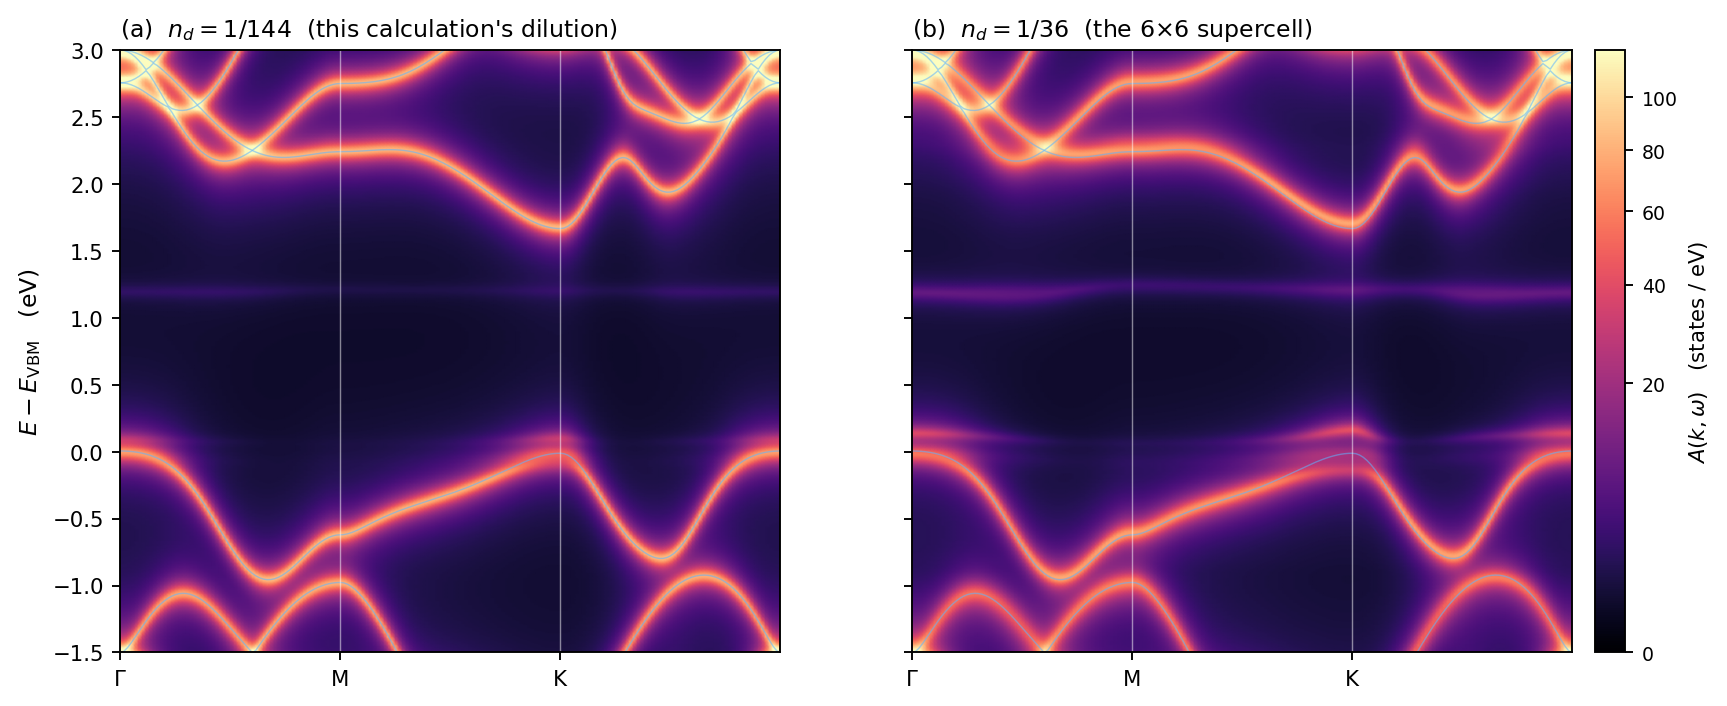
\includegraphics[width=\columnwidth]{kpath_spectral.png}
  \caption{Electron--defect spectral function $A(\kk,\omega)$ along
  $\Gamma$--M--K--$\Gamma$ for the relaxed sulfur vacancy, at two
  concentrations, with the bare interpolated bands overlaid. The flat in-gap
  lines are the Koster--Slater bound states; their energy is $\kk$-independent
  by construction while their weight is not.}
  \label{fig:akw}
\end{figure}

\begin{figure*}[t]
  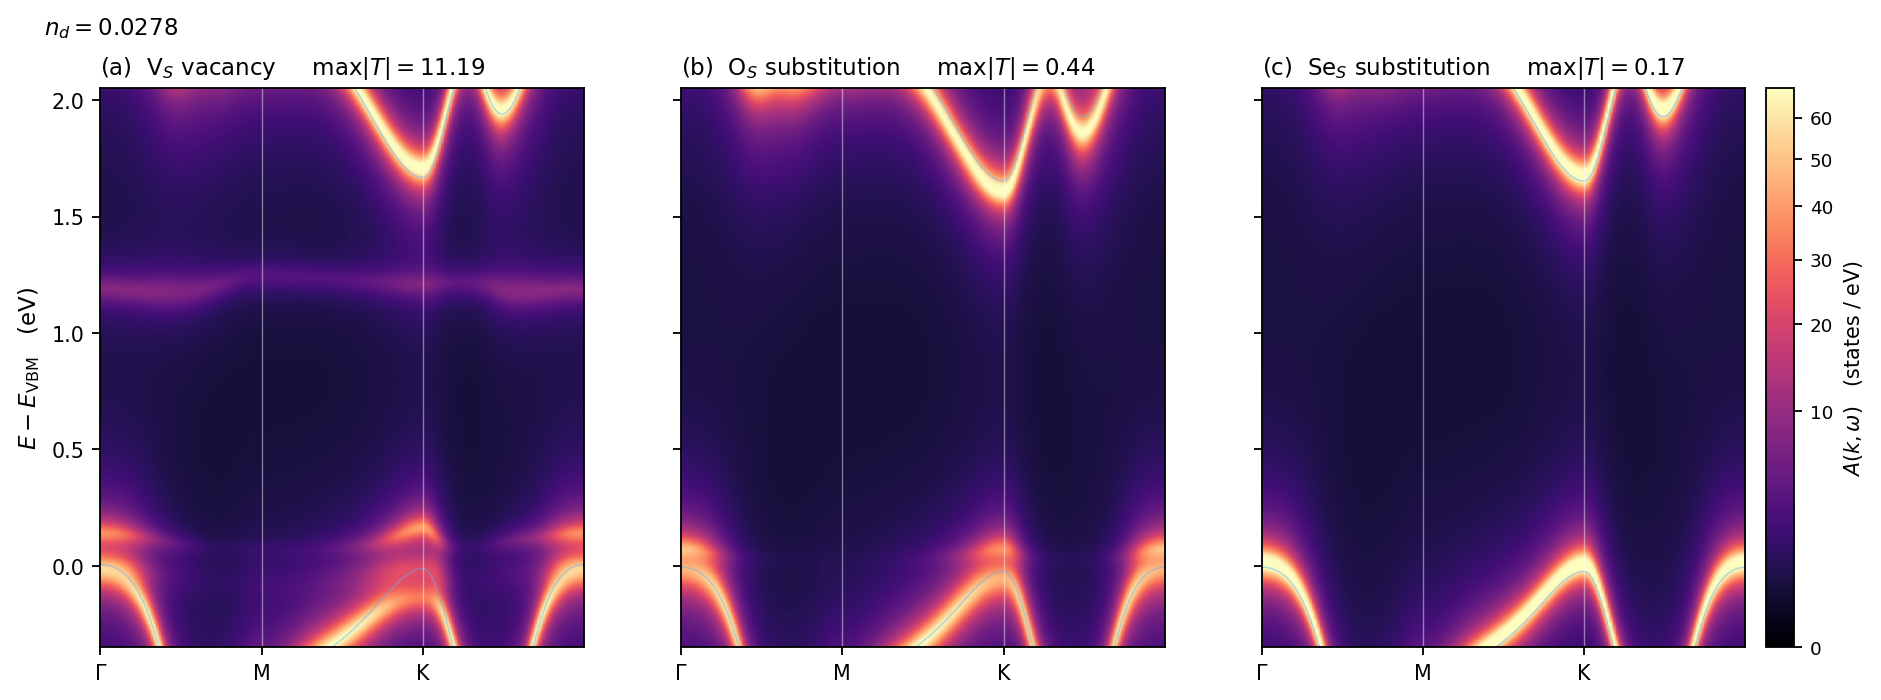
\includegraphics[width=\textwidth]{three_defects.png}
  \caption{The same pipeline applied to three point defects at
  $n_d = 1/36$: identical chains ($16$ blocks, $141$ min), identical transform,
  identical cluster. A bound state requires $1 - \mathcal{V}\mathcal{G}^A$ to
  become singular in the gap, where $\mathcal{G}^A$ is real; only the vacancy
  achieves it. The isovalent substitutions leave the gap clean and merely
  broaden the host bands, strongly for O$_{\rm S}$ and barely at all for
  Se$_{\rm S}$.}
  \label{fig:three}
\end{figure*}


\subsection{Application}

Figure~\ref{fig:three} shows the method applied unchanged to three point
defects. The chains are indistinguishable in cost ($16$ blocks, $141$ min,
operator identity $2\times10^{-11}$ to $7\times10^{-12}$) because the cost
depends only on the mesh and manifold dimensions, not on $\dV$. The physics is
not: the vacancy drives $\max|T| = 11.2$ and binds two in-gap states, whereas
the isovalent substitutions reach only $0.44$ and $0.17$ and bind none. Since
$\mathcal{G}^A$ is real in the gap, the absence of a singularity in
$1 - \mathcal{V}\mathcal{G}^A$ is a statement, not a numerical near-miss.


\section{Validation}
\label{sec:validation}

Each stage is gated separately, so that a failure is localized rather than
absorbed into a final discrepancy. Table~\ref{tab:validation} collects the
results.

\subsection{Operator level}

The application of $\dV$ inside the Lanczos recursion,
Eq.~\eqref{eq:applydV}, is compared against the independently constructed
vertex matrix by projecting the operator applied to known band states onto the
band basis. The two paths share no code beyond the potential file. Agreement is
$2\times10^{-11}$ relative on the $12\times12$ mesh and $2\times10^{-14}$ on
$6\times6$; the test is run at the start of every production chain and is the
gate for any change to the fold.

\subsection{Against a supercell reference}
\label{sec:truth}

The coset construction of Sec.~\ref{sec:freegrid} makes a supercell comparison
possible at more than one supercell $k$-point while holding the concentration
fixed. The three $M$ cosets are symmetry-equivalent and the downfolding does not
know it: run separately they return quasiparticle levels agreeing to every
printed digit, matching the exact degeneracy of the supercell reference. A
dedicated $107$-atom calculation at the three $M$ points supplies a reference no
part of the downfolding has seen.

Levels agree with a rigid offset: $+25.5 \pm 1.7\meV$ at $\Gamma$ (5/5
features) and $+25.0 \pm 0.8\meV$ at $M$ (5/5). The two offsets agree to
$0.5\meV$ --- the constant is a property of $\dV$, not of $\kk$. It is a
potential-reference convention: $\dV$ is vacuum-aligned while the reference is
anchored on deep levels, and the difference is predicted with no fitting from
two independently measured quantities ($+17.9\meV$ here), leaving residuals of
$+7.6 \pm 1.7$ and $+7.1 \pm 0.8\meV$.

The same machinery bounds what is worth chasing. Running the finer mesh
directly rather than by cosets dilutes the defect four-fold with no change of
alignment (the same $\dV$, so the reference constant cancels exactly, and both
meshes contain the same high-symmetry points so the pristine edges are
identical). The true in-gap levels move by $-11.1$ and $+3.7\meV$: the
supercell reference itself carries $4$--$11\meV$ of periodic-image error, of
the same size as the residual above.

\subsection{End to end}

Finally the assembled chain --- Wannier gauge, pair kernel, cluster truncation,
fine-mesh $\mathcal{G}^A$, Dyson solve --- is closed onto the coarse-mesh
result. The deep in-gap bound state, a root of a determinant with no $\kk$ in
it, comes out at $+1.2019$ eV against $+1.2023$ eV from direct diagonalization
of $H_{\rm eff}(\omega)$: $0.38\meV$. A systematic error anywhere in the chain
could not survive this comparison.

A second in-gap feature $68\meV$ above the valence edge differs by $7.3\meV$,
and doubling the frequency resolution moves it by only $1.5\meV$, so it is not a
grid artefact. At $\eta = 50\meV$ that state is hybridized with the valence
continuum: it is a resonance, and the peak of $|T|$ is not the same quantity as
a quasiparticle fixed point computed on a discrete coarse spectrum that has no
continuum to hybridize with.

\begin{table}[t]
\caption{Validation summary. Energies in meV unless noted.}
\label{tab:validation}
\begin{ruledtabular}
\begin{tabular}{lll}
Stage & Test & Result \\
\colrule
Fold          & $C_3$ degeneracy on commensurate grid & $0$--$4\,\mu$eV \\
Vertex        & operator identity, $12\times12$        & $2\times10^{-11}$ \\
Vertex        & operator identity, $6\times6$          & $2\times10^{-14}$ \\
Vertex        & direct vs.\ coset-diagonal blocks      & $2\times10^{-6}$ \\
Chain         & $N_S$ convergence ($16 \to 24$)        & $0.8$ \\
Downfold      & vs.\ supercell at $\Gamma$ (5/5)       & $+7.6 \pm 1.7$ \\
Downfold      & vs.\ supercell at $M$ (5/5)            & $+7.1 \pm 0.8$ \\
Reference     & periodic-image error of the reference  & $4$--$11$ \\
$\omega$ fit  & held-out node                          & $0.026$ \\
$\omega$ fit  & quasiparticle fixed points             & $0.201$ \\
Interpolation & leave-one-out, bare vertex (median)    & $0.744$ \\
Interpolation & leave-one-out, dressed vertex          & $0.61$--$0.88$ \\
End to end    & cluster vs.\ direct, deep level        & $0.38$ \\
\end{tabular}
\end{ruledtabular}
\end{table}


\section{Computational parameters, scaling and cost}
\label{sec:cost}

\subsection{Parameters}

Ground state and pristine band structure with
\textsc{Quantum ESPRESSO}~\cite{QE2009,QE2017}, PBE~\cite{PBE1996},
$E_{\rm cut}^{\rm wfc} = 50$ Ry, $E_{\rm cut}^{\rho} = 200$ Ry, a $2$D
truncated Coulomb treatment, and a $24$~\AA{} vacuum. The defect supercell is
$6\times6$ ($107$--$108$ atoms), relaxed. The pristine calculation supplying the
active manifold uses a $27\times27\times216$ FFT grid, $20$ bands and a
$12\times12$ $k$-mesh; the potential is band-limited to
$162\times162\times216$ per Sec.~\ref{sec:vertex}. The active manifold is the
$11$-band $d+p$ group, $N_A = 1584$. Chains use $N_S = 16$ blocks at
$12\times12$ and $N_S = 24$ at $6\times6$. Wannier functions from
\textsc{Wannier90}~\cite{Wannier90}, $11$ per cell, Mo-$d$ and S-$p$
projections, no disentanglement. The $T$-matrix uses a cluster radius $4a$
($61$ cells, dimension $671$), a $96\times96$ mesh for
Eq.~\eqref{eq:GA_fine}, and $\eta = 50\meV$.

Note that a host calculation must declare every atomic species appearing in any
defect cell, including species absent from the pristine cell, since the
nonlocal projector count is indexed by the \emph{cell's} species list.

\subsection{Scaling}

At fixed rank count the vertex application, Eq.~\eqref{eq:applydV}, costs
\begin{equation}
  t_{\rm fold} \;\propto\; \frac{N_r\, n_b\, N_k^{3}}{n_{\rm pool}},
\end{equation}
an $N_k^2$ channel double loop times $N_k$ columns per rank; full
reorthogonalization carries the same $N_k^3$ with an additional $N_S^2$.
Measured, $36 \to 144$ $k$-points take the multiply from $4.1$ to $261$~s,
i.e.\ $64\times = 4^3$, confirming the law. Memory scales as $N_k^2$, which is
what limits the chain length. Reorthogonalization overtakes the vertex
application around the ninth block.

Storing every block is what caps the chain length, so it is worth testing
whether it is needed. Repeating an $N_S=24$ chain while orthogonalizing against
only the last $m$ blocks gives, for $m = 2, 4, 8$ and for full: an orthogonality
$\max_{ij}\lVert Q_i^\dagger Q_j-\delta_{ij}\rVert = 6.04\times10^{-9}$
\emph{identical to four figures}, bit-identical levels, chain matrices differing
by $3\times10^{-14}$ on a scale of $31$, and zero Ritz values in the gap in every
case. Full reorthogonalization does nothing here, for the reason the theory
gives: loss of orthogonality is triggered by a converged Ritz value, and $24$
blocks of width $396$ in $\sim10^6$ dimensions converge none. (The residual
$\sqrt\epsilon$ is the single-pass classical Gram--Schmidt within a step, not a
recurrence loss.) The gain is memory rather than speed --- $1.65\times$ faster,
but $Q_s$ falls from $N_S+1$ blocks to two, i.e.\ $531 \to 62$ GB here and
$2.12$ TB $\to 250$ GB with spin--orbit coupling, which moves an SOC
$12\times12$ calculation from eight nodes onto one. The scope is what was
measured: a longer chain, or a spectrum that lets a Ritz value converge, would
behave differently, so the implementation of record should be \emph{partial}
reorthogonalization --- monitor the orthogonality, which is cheap, and
reorthogonalize fully only when it degrades.

\subsection{Cost}

On one $128$-core node: the $144$-$k$ chain takes $140$ min ($16$ blocks,
$261$~s per block in the vertex application). Post-processing is dominated by
the continued fraction, $6$~s per frequency at $N_A = 1584$, $N_S = 16$; the
cluster solve and the pair-Wannier transform are $0.5$~s and $0.1$~s per
frequency. Frequencies are independent, and an interleaved eight-worker split
delivers $450$ frequencies in $6$~min $25$~s ($0.85$~s per frequency, a
$13.9\times$ speedup). The complete spectral function of
Fig.~\ref{fig:akw} --- $450$ frequencies, $181$ $k$-points --- therefore costs
minutes once the chain exists, and any defect concentration afterwards is free
because $T$ is independent of $n_d$.


\begin{acknowledgments}
Computations were performed on Anvil at Purdue University.
\end{acknowledgments}

\begin{thebibliography}{99}

\bibitem{Feshbach1958} H.~Feshbach, Ann.\ Phys.\ (N.Y.) \textbf{5}, 357 (1958).

\bibitem{Lowdin1951} P.-O.~L\"owdin, J.\ Chem.\ Phys.\ \textbf{19}, 1396 (1951).

\bibitem{KosterSlater1954} G.~F.~Koster and J.~C.~Slater,
Phys.\ Rev.\ \textbf{95}, 1167 (1954).

\bibitem{Haydock1972} R.~Haydock, V.~Heine, and M.~J.~Kelly,
J.\ Phys.\ C \textbf{5}, 2845 (1972).

\bibitem{MarzariVanderbilt1997} N.~Marzari and D.~Vanderbilt,
Phys.\ Rev.\ B \textbf{56}, 12847 (1997).

\bibitem{SouzaMarzariVanderbilt2001} I.~Souza, N.~Marzari, and D.~Vanderbilt,
Phys.\ Rev.\ B \textbf{65}, 035109 (2001).

\bibitem{MarzariRMP2012} N.~Marzari, A.~A.~Mostofi, J.~R.~Yates, I.~Souza, and
D.~Vanderbilt, Rev.\ Mod.\ Phys.\ \textbf{84}, 1419 (2012).

\bibitem{Giustino2007} F.~Giustino, M.~L.~Cohen, and S.~G.~Louie,
Phys.\ Rev.\ B \textbf{76}, 165108 (2007).

\bibitem{LuBernardi2020} I.-T.~Lu, J.~Park, J.-J.~Zhou, and M.~Bernardi,
npj Comput.\ Mater.\ \textbf{6}, 29 (2020).

\bibitem{QE2009} P.~Giannozzi \textit{et al.},
J.\ Phys.: Condens.\ Matter \textbf{21}, 395502 (2009).

\bibitem{QE2017} P.~Giannozzi \textit{et al.},
J.\ Phys.: Condens.\ Matter \textbf{29}, 465901 (2017).

\bibitem{Wannier90} G.~Pizzi \textit{et al.},
J.\ Phys.: Condens.\ Matter \textbf{32}, 165902 (2020).

\bibitem{PBE1996} J.~P.~Perdew, K.~Burke, and M.~Ernzerhof,
Phys.\ Rev.\ Lett.\ \textbf{77}, 3865 (1996).

\end{thebibliography}

\end{document}
